% Options for packages loaded elsewhere
\PassOptionsToPackage{unicode}{hyperref}
\PassOptionsToPackage{hyphens}{url}
%
\documentclass[
  11pt,
]{article}
\usepackage{amsmath,amssymb}
\usepackage{iftex}
\ifPDFTeX
  \usepackage[T1]{fontenc}
  \usepackage[utf8]{inputenc}
  \usepackage{textcomp} % provide euro and other symbols
\else % if luatex or xetex
  \usepackage{unicode-math} % this also loads fontspec
  \defaultfontfeatures{Scale=MatchLowercase}
  \defaultfontfeatures[\rmfamily]{Ligatures=TeX,Scale=1}
\fi
\usepackage{lmodern}
\ifPDFTeX\else
  % xetex/luatex font selection
\fi
% Use upquote if available, for straight quotes in verbatim environments
\IfFileExists{upquote.sty}{\usepackage{upquote}}{}
\IfFileExists{microtype.sty}{% use microtype if available
  \usepackage[]{microtype}
  \UseMicrotypeSet[protrusion]{basicmath} % disable protrusion for tt fonts
}{}
\makeatletter
\@ifundefined{KOMAClassName}{% if non-KOMA class
  \IfFileExists{parskip.sty}{%
    \usepackage{parskip}
  }{% else
    \setlength{\parindent}{0pt}
    \setlength{\parskip}{6pt plus 2pt minus 1pt}}
}{% if KOMA class
  \KOMAoptions{parskip=half}}
\makeatother
\usepackage{xcolor}
\usepackage[margin=1in]{geometry}
\usepackage{longtable,booktabs,array}
\usepackage{calc} % for calculating minipage widths
% Correct order of tables after \paragraph or \subparagraph
\usepackage{etoolbox}
\makeatletter
\patchcmd\longtable{\par}{\if@noskipsec\mbox{}\fi\par}{}{}
\makeatother
% Allow footnotes in longtable head/foot
\IfFileExists{footnotehyper.sty}{\usepackage{footnotehyper}}{\usepackage{footnote}}
\makesavenoteenv{longtable}
\usepackage{graphicx}
\makeatletter
\def\maxwidth{\ifdim\Gin@nat@width>\linewidth\linewidth\else\Gin@nat@width\fi}
\def\maxheight{\ifdim\Gin@nat@height>\textheight\textheight\else\Gin@nat@height\fi}
\makeatother
% Scale images if necessary, so that they will not overflow the page
% margins by default, and it is still possible to overwrite the defaults
% using explicit options in \includegraphics[width, height, ...]{}
\setkeys{Gin}{width=\maxwidth,height=\maxheight,keepaspectratio}
% Set default figure placement to htbp
\makeatletter
\def\fps@figure{htbp}
\makeatother
\setlength{\emergencystretch}{3em} % prevent overfull lines
\providecommand{\tightlist}{%
  \setlength{\itemsep}{0pt}\setlength{\parskip}{0pt}}
\setcounter{secnumdepth}{5}
\setlength\parindent{24pt}
\usepackage{float}
\usepackage{flafter}
\usepackage{pdflscape}
\usepackage{rotating}
\usepackage{booktabs}
\usepackage{longtable}
\usepackage{array}
\usepackage{multirow}
\usepackage{wrapfig}
\usepackage{float}
\usepackage{colortbl}
\usepackage{pdflscape}
\usepackage{tabu}
\usepackage{threeparttable}
\usepackage{threeparttablex}
\usepackage[normalem]{ulem}
\usepackage{makecell}
\usepackage{xcolor}
\ifLuaTeX
  \usepackage{selnolig}  % disable illegal ligatures
\fi
\IfFileExists{bookmark.sty}{\usepackage{bookmark}}{\usepackage{hyperref}}
\IfFileExists{xurl.sty}{\usepackage{xurl}}{} % add URL line breaks if available
\urlstyle{same}
\hypersetup{
  pdftitle={Experiment Status Quo Applications},
  pdfauthor={Omar Vasquez Duque},
  hidelinks,
  pdfcreator={LaTeX via pandoc}}

\title{Experiment Status Quo Applications}
\usepackage{etoolbox}
\makeatletter
\providecommand{\subtitle}[1]{% add subtitle to \maketitle
  \apptocmd{\@title}{\par {\large #1 \par}}{}{}
}
\makeatother
\subtitle{Analysis July 19}
\author{Omar Vasquez Duque}
\date{}

\begin{document}
\maketitle

\hypertarget{method}{%
\section{Method}\label{method}}

\hypertarget{experimental-design}{%
\subsection{Experimental Design}\label{experimental-design}}

The data come from two experiments the author ran on Prolific between July 13 and July 14, 2023. Both were trivia games in which the participants had to look for the answers to either 6 or 5 questions (available in the Appendix). The respondents were incentivized to find the correct answers. The regular compensation was \$1 for a 6-minute task, and every participant that found the 5 or 6 correct answers doubled her compensation to \$2. In the first experiment, half of the questions were about popular culture and the other half about weather forecasts. This design intended to compare possible status quo effects in search with those of weather applications. The second experiment focused solely on search engines.

There were two experimental conditions in each study: (i) a \emph{forced-choice condition}, in which each participant chose a search engine and/or a weather application, and (ii) a \emph{default condition}, in which each participant was assigned to a search engine and/or weather application by default. The possible defaults were Google, Bing, Yahoo, and DuckDuck Go for search; and the Weather Channel, AccuWeather, and WeatherUnderground for weather forecasts.\footnote{For search, there was an equal probability of being assigned to the forced choice or default condition. In the weather applications part, a 25\% chance of either having to choose an app, and a 25\% of being assigned to one of the three defaults. The difference is because the author did not have a strong prior about status quo effects in weather applications.}

In the first study, each participant was randomly assigned to one of the conditions in each part (i.e.search and weather forecasts). This means a participant could have been assigned to the forced choice condition in the first half of the study and then to a default condition in the second one. The second study focused solely on search. Thus, the five questions presented there were about popular culture. Nonetheless, the author included an additional manipulation in the second study that did not have any effect on the outcomes. Said failed manipulation was the addition of a video the participants had to watch right before seeing the first question, which intended to manipulate people's attention. In both studies, the participants read a multiple choice question and right after responding they had to report what application(s) they had used to find the answer.

\hypertarget{sample}{%
\subsection{Sample}\label{sample}}

Prolific recruited 344 people to participate in the first experiment, and 416 in the second one. After filtering the responses of those who did not pass attention checks, did not complete the questionnaire, and responded either 50\% below or 175\% above the median completion time, the final sample sample sizes lower to 257 and 319 for the first and second experiments, respectively. The only two restrictions that applied to the participant poll were that they needed to reside in the U.S. and be fluent in English. Both samples were highly educated. Most of the respondents had a college degree. The mean age of the participants was 38 in the first experiment and 42 in the second one. Almost half of the participants identified as female and the rest as male. Slightly below 5\% of the samples identified as non-binary or preferred not to respond the question. The Appendix contains two tables displaying descriptive statistics and performing a balance test among the experimental conditions.

\hypertarget{results}{%
\section{Results}\label{results}}

\hypertarget{most-of-the-participants-clearly-preferred-the-dominant-search-engine-but-the-preferences-for-weather-applications-were-divided}{%
\subsection{Most of the participants clearly preferred the dominant search engine but the preferences for weather applications were divided}\label{most-of-the-participants-clearly-preferred-the-dominant-search-engine-but-the-preferences-for-weather-applications-were-divided}}

Figure \ref{fig:preferences} below shows the participants' preferences when forced to choose. This is the normative benchmark that discards any potential exploitation of the users' inertia. In search, Google's dominance is clear. Eighty nine percent of the participants chose it. DuckDuck Go ranks second with a mere 8\% of the users' preferences. In contrast, the two most popular weather applications showed a more similar share of preferences. The Weather Channel ranks first with 55\% of the choices, AccuWeather followed it with 35\%, and Weather Underground ranked last with roughly 10\% of the preferences.

\begin{figure}

{\centering 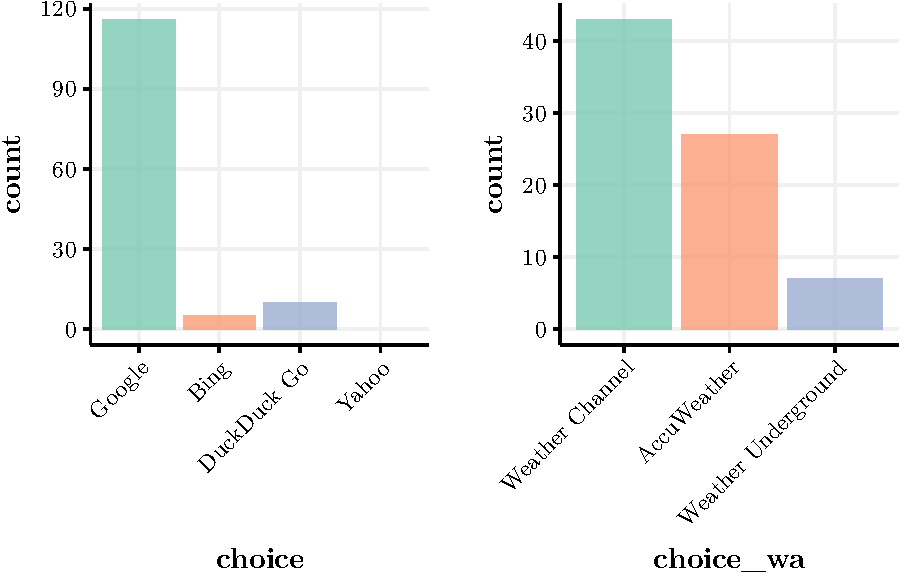
\includegraphics[width=0.7\textwidth]{Results-July19-307_files/figure-latex/preferences-1} 

}

\caption{Preferences for Search Engines and Weather Apps}\label{fig:preferences}
\end{figure}

\hypertarget{strong-status-quo-effects-in-search-and-weather-applications}{%
\subsection{Strong status quo effects in search and weather applications}\label{strong-status-quo-effects-in-search-and-weather-applications}}

A status quo effect refers to the disparity in market share that an application would possess when it is set as the user's default option, as opposed to when the user is compelled to make a choice. This is formally represented as \(Pa_i|D_i - Pa_i|C\), where \(Pa_i|D_i\) is the probability of choosing application \(a\) when it is the default, and \(Pa_i|C\) is the probability of choosing the same application when its users are forced to choose their preferred option.

The statistical analysis of this section appraises status quo effects benefiting Bing, DuckDuckGo, the Weather Channel, AccuWeather, and Weather Underground. Yahoo's case is then reported with a mere frequency table. This is because no participant chose Yahoo in the forced choice condition, which makes the statistical analysis impossible.

As just noted, most of the respondents in the forced choice condition chose Google. Only a few chose Bing (4\%), and 8\% chose DuckDuck Go. However, when the participants were assigned to any rival of Google by default, a very substantial part of the respondents used the default, and not only in the first question but also in the third one. Ninety percent of those assigned to DuckDuck Go used it in question 1, compared to 80\% of those assigned to Bing, and 60\% of those assigned to Yahoo. The effect lowered by roughly 10\% in question 3. The following plots show the operationalization of status quo effects with forced choice as the benchmark. Google is the only search engine that does not directly benefit from its default position. This is because its share of preferences does not change substantially when it is people's default and when users are forced to choose.

The weather application data show a similar effect. Figure \ref{fig:Sqweather} displays the three applications show a much higher use rate when they are assigned as people's default than when people are forced to choose. Weather Underground was the least sticky default. Fewer people stuck to it in question 1, and more switched to another application by question 3.

\begin{figure}

{\centering 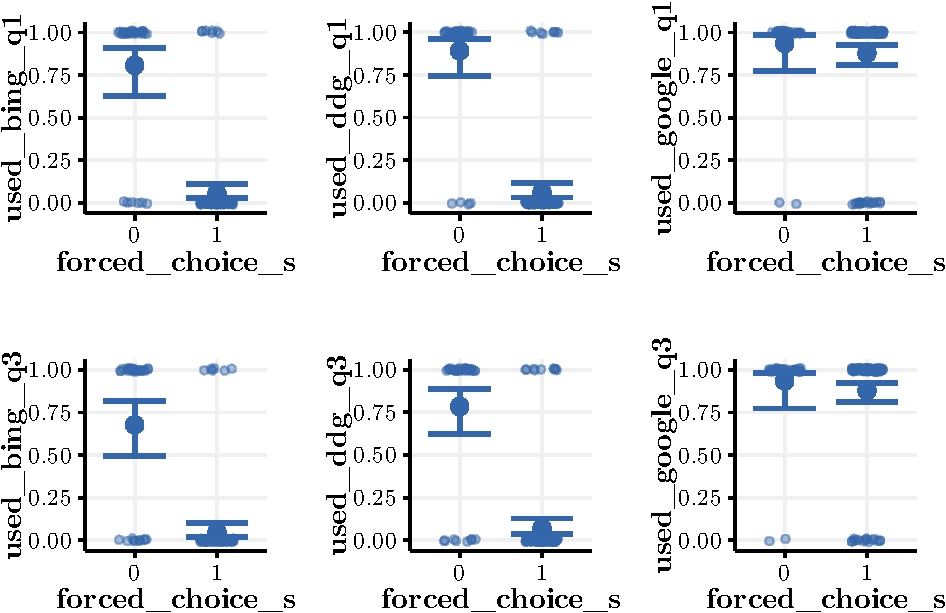
\includegraphics[width=0.7\textwidth]{Results-July19-307_files/figure-latex/Sqsearch-1} 

}

\caption{Status Quo Search Engines}\label{fig:Sqsearch}
\end{figure}

\begin{figure}

{\centering 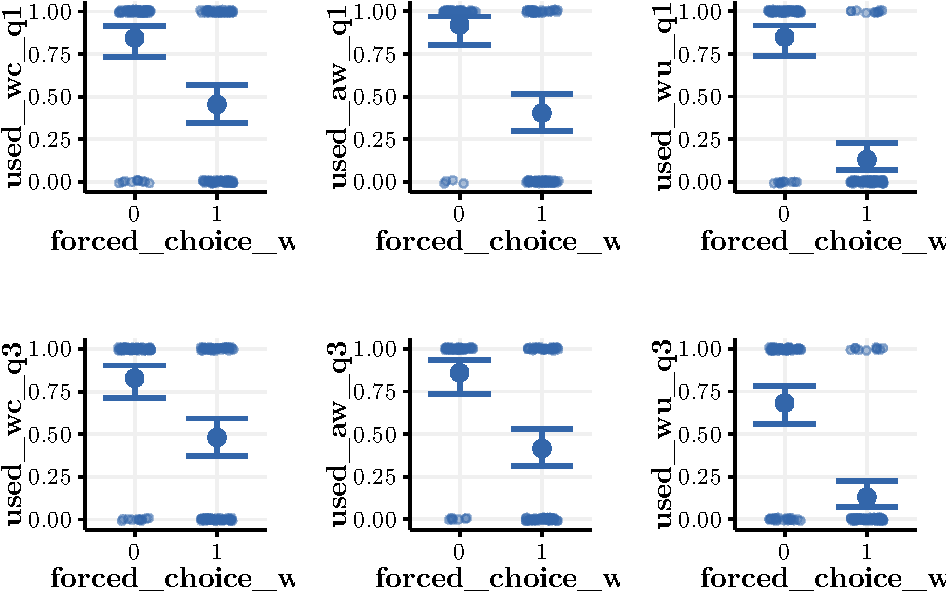
\includegraphics[width=0.7\textwidth]{Results-July19-307_files/figure-latex/Sqweather-1} 

}

\caption{Status Quo Weather Apps}\label{fig:Sqweather}
\end{figure}

\hypertarget{downward-trend-of-default-effects-in-search}{%
\subsection{Downward Trend of Default Effects in Search}\label{downward-trend-of-default-effects-in-search}}

Bing and Yahoo exhibited stronger default effects in question 1 than question 3. This was also the Weather Underground's case. This trend motivated the author to run a follow-up experiment with five questions, in which there was just a default condition. In this second experiment, the participants were randomly assigned to Google or Bing by default (with an equal probability). Figure \ref{fig:Bing1v5} shows how Bing's default effect goes down from roughly 75\% in question 1 to 50\% in question 5 (McNemar's Chi-squared test p \textless{} 0.01).

Relatedly, the use of Google when Bing is the default increases substantially comparing question 1 and question 5. While only a quarter of the participants assigned to Bing by default used Google in question one, almost half did so to find the answer to the last question.

\begin{figure}

{\centering 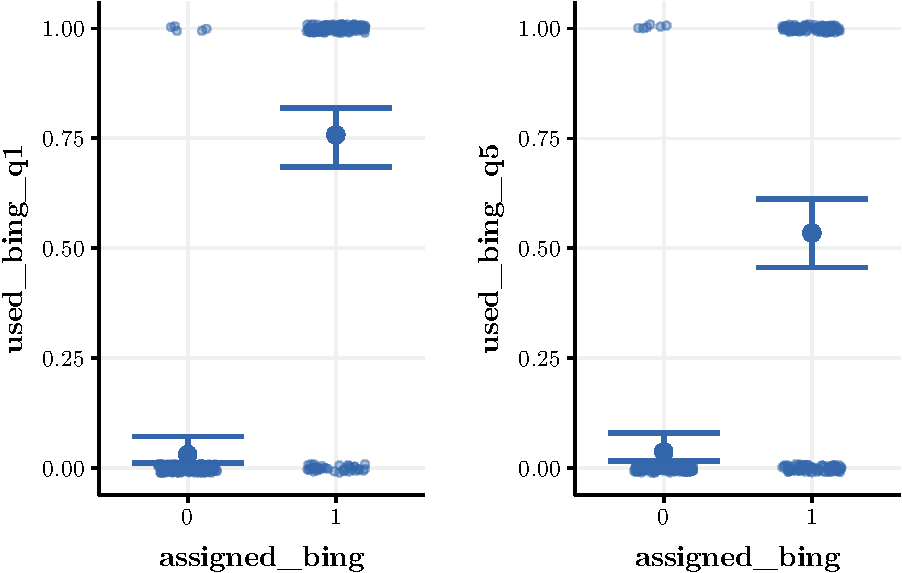
\includegraphics[width=0.6\textwidth]{Results-July19-307_files/figure-latex/Bing1v5-1} 

}

\caption{Status Quo Bing Q1 and Q5}\label{fig:Bing1v5}
\end{figure}

\begin{figure}

{\centering 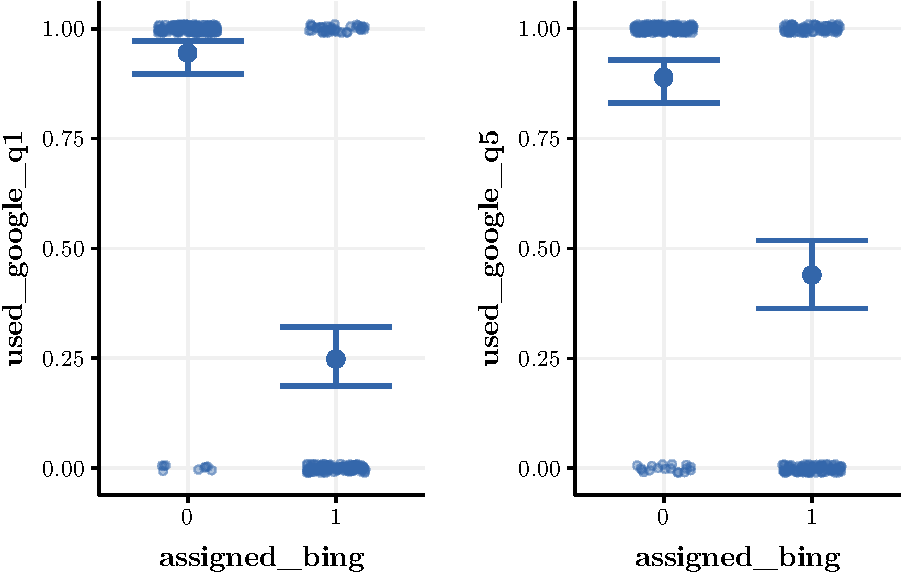
\includegraphics[width=0.6\textwidth]{Results-July19-307_files/figure-latex/GoogBD1v5-1} 

}

\caption{Use of Google When Bing is the Default Q1 and Q5}\label{fig:GoogBD1v5}
\end{figure}

\hypertarget{googles-use-goes-down-when-another-search-engine-is-the-users-default}{%
\subsection{Google's Use Goes Down When Another Search Engine is the Users' Default}\label{googles-use-goes-down-when-another-search-engine-is-the-users-default}}

As noted, Google does not benefit from a default effect. However, Google's rivals do. And when a rival of Google increases its use, Google's use goes down. In fact, only roughly 20\% of the participants used Google to find the answer to the first question when assigned to any of Google's rivals by default. However, the number goes up to 32\% in question 3. Figure \ref{fig:Sqsearchb} shows this effect. It also shows that Google was the only option the participants tended to use in addition to their default.

{[}Check what happened experiment 2{]}

\begin{verbatim}
\end{verbatim}

Now, do the same for Q5

See how this effect affects Google

Mind there are two ways to operationalize the effect:

\begin{enumerate}
\def\labelenumi{\arabic{enumi})}
\item
  compared with choice-screen
\item
  compared with any other default
\end{enumerate}

\begin{figure}

{\centering 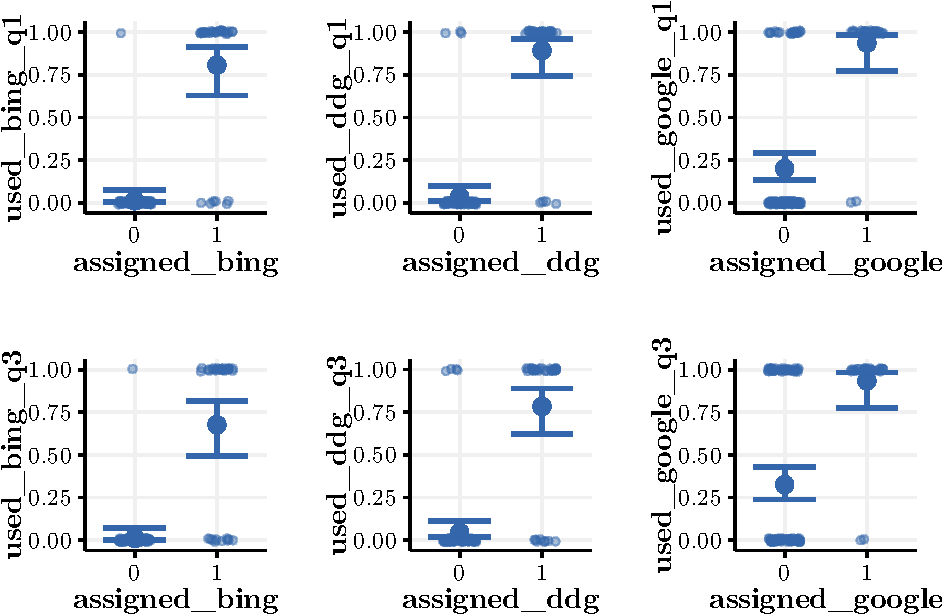
\includegraphics[width=0.65\textwidth]{Results-July19-307_files/figure-latex/Sqsearchb-1} 

}

\caption{Search Engine Use. default vs. Other as Default}\label{fig:Sqsearchb}
\end{figure}

\hypertarget{default-affects-peoples-perceptions-about-the-quality-of-each-application}{%
\subsection{Default affects people's perceptions about the quality of each application}\label{default-affects-peoples-perceptions-about-the-quality-of-each-application}}

\hypertarget{video-had-no-effect.-probably-everyone-paid-attention.-check-number-of-correct-answers}{%
\subsection{Video had no effect. Probably everyone paid attention. Check number of correct answers}\label{video-had-no-effect.-probably-everyone-paid-attention.-check-number-of-correct-answers}}

See if video had an effect\ldots{} It did not work out. No difference

Substantial effect! lowers use of Google!

\hypertarget{big-regression-general-analysis-status-quo-effect}{%
\subsection{Big regression general analysis status quo effect}\label{big-regression-general-analysis-status-quo-effect}}

There si something wrong with the default data set. Showing NAs in assigned to a

Data defaults without Google

Interesting coefficients, qualitatively. Now, run glm because p\textgreater1

\hypertarget{check-if-those-who-use-the-default-use-another-one-too}{%
\subsection{Check if those who use the default use another one too!}\label{check-if-those-who-use-the-default-use-another-one-too}}

This is important. q1 only a few use more than one, q3 many more explore.

Code below irrelevant. q1 only one person used more than one

Code above is not what I need. The relevant variable is stat\_quo\_qi * just\_one\_qi

\hypertarget{now-with-the-second-experiment}{%
\subsubsection{Now with the second experiment}\label{now-with-the-second-experiment}}

Interesting result. More people tend to use Bing exclusively over time.

\hypertarget{results-weather-apps}{%
\section{Results Weather Apps}\label{results-weather-apps}}

One plot for sq q1 for each (a1\_q1, a2\_q1, a3\_q1)

Another for sq q3 for each (a1\_q3, a2\_q3, a3\_q3)

Effect\_plot to show correlations browsers/s.engines controlling for changes in OSX market shares

\hypertarget{appendix}{%
\section{Appendix}\label{appendix}}

\begin{table}[!htbp] \centering \renewcommand*{\arraystretch}{1.1}\caption{Summary Statistics}\resizebox{\textwidth}{!}{
\begin{tabular}{lrrrrrrl}
\hline
\hline
choice\_search & \multicolumn{3}{c}{0} & \multicolumn{3}{c}{1} &   \\ 
 Variable & \multicolumn{1}{c}{N} & \multicolumn{1}{c}{Mean} & \multicolumn{1}{c}{SD} & \multicolumn{1}{c}{N} & \multicolumn{1}{c}{Mean} & \multicolumn{1}{c}{SD} & \multicolumn{1}{c}{Test} \\ 
\hline
age & 126 & 38 & 12 & 131 & 37 & 13 & F$=0.604^{}$ \\ 
education & 126 &  &  & 131 &  &  & X2$=2.313^{}$ \\ 
... college degree & 45 & 36\% &  & 57 & 44\% &  &  \\ 
... graduate degree & 24 & 19\% &  & 19 & 15\% &  &  \\ 
... high school & 19 & 15\% &  & 20 & 15\% &  &  \\ 
... some college & 36 & 29\% &  & 34 & 26\% &  &  \\ 
... some high-school & 2 & 2\% &  & 1 & 1\% &  &  \\ 
computer\_use & 126 &  &  & 131 &  &  & X2$=5.285^{}$ \\ 
... between 2-4 hours/day & 24 & 19\% &  & 29 & 22\% &  &  \\ 
... between 4-6 hours/day & 31 & 25\% &  & 20 & 15\% &  &  \\ 
... between 6-8 hours/day & 27 & 21\% &  & 30 & 23\% &  &  \\ 
... more than 8 hours/day & 41 & 33\% &  & 44 & 34\% &  &  \\ 
... up to 2 hours/day & 3 & 2\% &  & 8 & 6\% &  &  \\ 
gender & 126 &  &  & 131 &  &  & X2$=1.793^{}$ \\ 
... female & 57 & 45\% &  & 66 & 50\% &  &  \\ 
... male & 65 & 52\% &  & 63 & 48\% &  &  \\ 
... non-binary & 3 & 2\% &  & 2 & 2\% &  &  \\ 
... prefer not to say & 1 & 1\% &  & 0 & 0\% &  &  \\ 
ethnicity & 126 &  &  & 131 &  &  & X2$=2.246^{}$ \\ 
... african american & 13 & 10\% &  & 8 & 6\% &  &  \\ 
... american indian & 12 & 10\% &  & 12 & 9\% &  &  \\ 
... asian & 1 & 1\% &  & 1 & 1\% &  &  \\ 
... hispanic & 10 & 8\% &  & 9 & 7\% &  &  \\ 
... other & 2 & 2\% &  & 1 & 1\% &  &  \\ 
... white & 88 & 70\% &  & 100 & 76\% &  & \\ 
\hline
\hline
\multicolumn{8}{l}{Statistical significance markers: * p<0.1; ** p<0.05; *** p<0.01}\\ 
\end{tabular}
}
\end{table}

\begin{table}[!htbp] \centering \renewcommand*{\arraystretch}{1.1}\caption{Summary Statistics}\resizebox{\textwidth}{!}{
\begin{tabular}{lrrrrrrl}
\hline
\hline
Bing\_default & \multicolumn{3}{c}{0} & \multicolumn{3}{c}{1} &   \\ 
 Variable & \multicolumn{1}{c}{N} & \multicolumn{1}{c}{Mean} & \multicolumn{1}{c}{SD} & \multicolumn{1}{c}{N} & \multicolumn{1}{c}{Mean} & \multicolumn{1}{c}{SD} & \multicolumn{1}{c}{Test} \\ 
\hline
age & 162 & 44 & 14 & 157 & 42 & 15 & F$=1.195^{}$ \\ 
education & 162 &  &  & 157 &  &  & X2$=3.527^{}$ \\ 
... college degree & 70 & 43\% &  & 68 & 43\% &  &  \\ 
... graduate degree & 29 & 18\% &  & 32 & 20\% &  &  \\ 
... high school & 17 & 10\% &  & 23 & 15\% &  &  \\ 
... some college & 45 & 28\% &  & 32 & 20\% &  &  \\ 
... some high-school & 1 & 1\% &  & 2 & 1\% &  &  \\ 
computer\_use & 162 &  &  & 157 &  &  & X2$=2.036^{}$ \\ 
... between 2-4 hours/day & 23 & 14\% &  & 30 & 19\% &  &  \\ 
... between 4-6 hours/day & 38 & 23\% &  & 31 & 20\% &  &  \\ 
... between 6-8 hours/day & 46 & 28\% &  & 41 & 26\% &  &  \\ 
... more than 8 hours/day & 42 & 26\% &  & 40 & 25\% &  &  \\ 
... up to 2 hours/day & 13 & 8\% &  & 15 & 10\% &  &  \\ 
gender & 162 &  &  & 157 &  &  & X2$=0.793^{}$ \\ 
... female & 79 & 49\% &  & 72 & 46\% &  &  \\ 
... male & 76 & 47\% &  & 80 & 51\% &  &  \\ 
... non-binary & 5 & 3\% &  & 4 & 3\% &  &  \\ 
... prefer not to say & 2 & 1\% &  & 1 & 1\% &  & \\ 
\hline
\hline
\multicolumn{8}{l}{Statistical significance markers: * p<0.1; ** p<0.05; *** p<0.01}\\ 
\end{tabular}
}
\end{table}

\end{document}
